% Options for packages loaded elsewhere
\PassOptionsToPackage{unicode}{hyperref}
\PassOptionsToPackage{hyphens}{url}
%
\documentclass[
  12pt,
]{article}
\usepackage{amsmath,amssymb}
\usepackage{lmodern}
\usepackage{iftex}
\ifPDFTeX
  \usepackage[T1]{fontenc}
  \usepackage[utf8]{inputenc}
  \usepackage{textcomp} % provide euro and other symbols
\else % if luatex or xetex
  \usepackage{unicode-math}
  \defaultfontfeatures{Scale=MatchLowercase}
  \defaultfontfeatures[\rmfamily]{Ligatures=TeX,Scale=1}
\fi
% Use upquote if available, for straight quotes in verbatim environments
\IfFileExists{upquote.sty}{\usepackage{upquote}}{}
\IfFileExists{microtype.sty}{% use microtype if available
  \usepackage[]{microtype}
  \UseMicrotypeSet[protrusion]{basicmath} % disable protrusion for tt fonts
}{}
\makeatletter
\@ifundefined{KOMAClassName}{% if non-KOMA class
  \IfFileExists{parskip.sty}{%
    \usepackage{parskip}
  }{% else
    \setlength{\parindent}{0pt}
    \setlength{\parskip}{6pt plus 2pt minus 1pt}}
}{% if KOMA class
  \KOMAoptions{parskip=half}}
\makeatother
\usepackage{xcolor}
\usepackage[margin=1in]{geometry}
\usepackage{graphicx}
\makeatletter
\def\maxwidth{\ifdim\Gin@nat@width>\linewidth\linewidth\else\Gin@nat@width\fi}
\def\maxheight{\ifdim\Gin@nat@height>\textheight\textheight\else\Gin@nat@height\fi}
\makeatother
% Scale images if necessary, so that they will not overflow the page
% margins by default, and it is still possible to overwrite the defaults
% using explicit options in \includegraphics[width, height, ...]{}
\setkeys{Gin}{width=\maxwidth,height=\maxheight,keepaspectratio}
% Set default figure placement to htbp
\makeatletter
\def\fps@figure{htbp}
\makeatother
\setlength{\emergencystretch}{3em} % prevent overfull lines
\providecommand{\tightlist}{%
  \setlength{\itemsep}{0pt}\setlength{\parskip}{0pt}}
\setcounter{secnumdepth}{-\maxdimen} % remove section numbering
\usepackage{fancyhdr}
\usepackage{fontspec}
\usepackage{xcolor}
\usepackage{hyperref}
\usepackage{pdfcomment}
\usepackage{datetime}
\usepackage[document]{ragged2e}
\usepackage{setspace}
\usepackage{subfig}

\setmainfont{Poppins}

\newdateformat{monthyeardate}{\monthname[\THEMONTH] \THEYEAR}

% header and footer
\fancypagestyle{firstpage}{
\setlength{\headheight}{75pt}
\setlength{\textheight}{600pt}
\fancyhead[C]{}
\fancyhead[L]{
\includegraphics{X:/DSA/Trends/equity/headers/PST_Equity_Edition-Trend_header.png}}
\fancyhead[R]{}

\fancyfoot[L]{\scriptsize{1011 Western Ave, Suite 500, Seattle WA 98104} \textcolor[HTML]{F05A28}. 206.464.7532 \textcolor[HTML]{F05A28}. www.psrc.org \textcolor[HTML]{F05A28}. \monthyeardate\today}
\fancyfoot[R]{\textcolor[HTML]{F05A28}\thepage}
\fancyfoot[C]{}
\renewcommand{\headrulewidth}{0pt}
\renewcommand{\footrulewidth}{4pt}
\renewcommand{\footrule}{\hbox to \headwidth{\color[HTML]{BCBEC0}\leaders\hrule height \footrulewidth\hfill}}
}

\fancypagestyle{otherpages}{
\fancyhead{}
\fancyfoot[L]{\scriptsize{1011 Western Ave, Suite 500, Seattle WA 98104} \textcolor[HTML]{F05A28}. 206.464.7532 \textcolor[HTML]{F05A28}. www.psrc.org \textcolor[HTML]{F05A28}. \monthyeardate\today}
\fancyfoot[R]{\textcolor[HTML]{F05A28}\thepage}
\fancyfoot[C]{}
\renewcommand{\headrulewidth}{0pt}
\renewcommand{\footrulewidth}{4pt}
\renewcommand{\footrule}{\hbox to \headwidth{\color[HTML]{BCBEC0}\leaders\hrule height \footrulewidth\hfill}}
}


\ifLuaTeX
  \usepackage{selnolig}  % disable illegal ligatures
\fi
\IfFileExists{bookmark.sty}{\usepackage{bookmark}}{\usepackage{hyperref}}
\IfFileExists{xurl.sty}{\usepackage{xurl}}{} % add URL line breaks if available
\urlstyle{same} % disable monospaced font for URLs
\hypersetup{
  pdftitle={Women and their Unique Travel Needs},
  pdfauthor={Suzanne Childress, Christy Lam, Mary Richards, Joanne Lin, Meg Grzybowski},
  hidelinks,
  pdfcreator={LaTeX via pandoc}}

\title{Women and their Unique Travel Needs}
\usepackage{etoolbox}
\makeatletter
\providecommand{\subtitle}[1]{% add subtitle to \maketitle
  \apptocmd{\@title}{\par {\large #1 \par}}{}{}
}
\makeatother
\subtitle{Data Gen: Exploring, Cleaning, Transforming (PUMS/OSPI data)}
\author{Suzanne Childress, Christy Lam, Mary Richards, Joanne Lin, Meg
Grzybowski}
\date{September 07, 2023}

\begin{document}
\maketitle

\hypertarget{title-of-article-womens-diverse-travel-needs-often-go-overlooked}{%
\section{Title of Article Women's Diverse Travel Needs Often Go
Overlooked}\label{title-of-article-womens-diverse-travel-needs-often-go-overlooked}}

\onehalfspacing

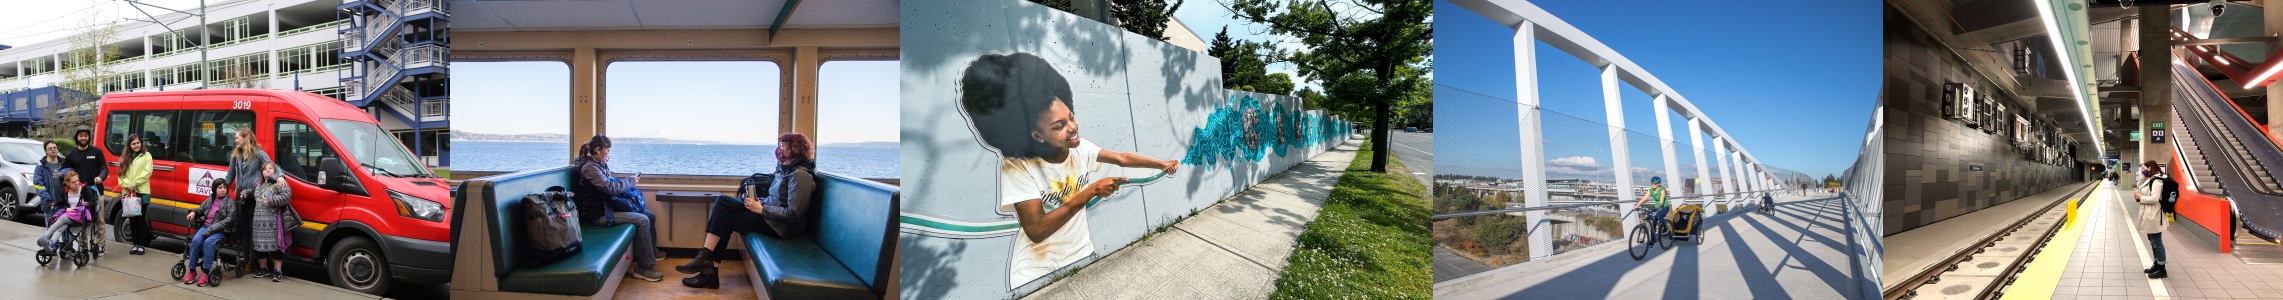
\includegraphics[width=1\textwidth,height=\textheight]{C:/GitHub/document-maker/templates/equity_example/women2_image_header.png}

\thispagestyle{firstpage}

\begin{flushleft}

\textbf{Subdivision - numbered sections
Divide your article into clearly defined and numbered sections. Subsections should be numbered 1.1 (then 1.1.1, 1.1.2, ...), 1.2, etc. (the abstract is not included in section numbering). Use this numbering also for internal cross-referencing: do not just refer to 'the text'. Any subsection may be given a brief heading. Each heading should appear on its own separate line.}

{\underline{\textbf{Keywords}}} women, non-binary, transportation, 

{\underline{\textbf{Abstract}}}

{\underline{\textbf{Acknowledgements}}}

{\underline{\textbf{1. Introduction}}}

Women have \href{http://libraryarchives.metro.net/DB_Attachments/2019-0294/UnderstandingHowWomenTravel_FullReport_FINAL.pdf}{\underline{\textcolor{blue}{transportation needs that have not historically been met}}} in urban environments.  The regional transportation system was traditionally designed around the need to quickly get to work at central locations at peak periods. Women tend to carry significantly more of the care-giving burdens of society and thus need a system that works \textbf{safely} for traveling with others to a variety of locations \textbf{at all times of day}. Women also represent a large portion of older populations who have unique transportation needs that are not well-served by our system built around driving and work destinations. Wome, especially women of color, are more likely to live in poverty and have lower earnings for the same jobs than men (Figure 3), which impacts many aspects of transportation needs.
\end{flushleft}

\begin{flushleft}
With the arrival of the COVID-19 pandemic, we saw a greater trend towards telecommuting for some people and continued trends in aging. Housing prices continue to soar and childcare options continue to degrade. With these new considerations at play, compounded with the existence on previous burdens on women, when will the transportation system evolve for women across diverse backgrounds?
\end{flushleft}

\newpage
\pagestyle{otherpages}
\setlength{\headheight}{10pt}
\setlength{\textheight}{665pt}
\fancyhead[L]{}

\{\underline{\textbf{Materials and Methods}}

\{\underline{\textbf{Theory}}

\hypertarget{puget-sound-regional-household-travel-survey}{%
\section{Puget Sound Regional Household Travel
Survey}\label{puget-sound-regional-household-travel-survey}}

\hypertarget{a-rich-data-source-for-travel-by-women}{%
\subsubsection{A rich data source for travel by
women}\label{a-rich-data-source-for-travel-by-women}}

\begin{flushleft}
The  \href{https://www.psrc.org/our-work/household-travel-survey-program}{\underline{\textcolor{blue}{PSRC regional household travel survey }}} contains detailed information about travel behaviors by race, ethnicity, gender, income, and location. The rich travel survey data source reveals the diversity women's experiences of travel throughout the region. Through the analysis of the regional household travel survey in this report, key trends have emerged that differentiate women resident's travel patterns from men's travel patterns across all modes. The 2017, 2019, and 2021 household travel surveys collected day-to-day information from households in the central Puget Sound region, such as how we traveled, where we went, how long it took—even where we chose to live and whether we got home deliveries, prior to COVID-19 and after.


This report starts with comparing travel by gender, during the stable period prior to COVID-19, and then dives into some broader, national trends, and finishes by taking a glance at recent trends that occurred in 2021, during COVId-19. Data from 2017 and 2019 have combined to give a more robust sample size.  You can also \href{https://household-travel-survey-psregcncl.hub.arcgis.com}{\underline{\textcolor{blue}{view the full dataset here}}}, including 2017, 2019 and 2021 data. 
\end{flushleft}

\hypertarget{travel-demands-put-different-pressures-on-women}{%
\subsubsection{Travel demands put different pressures on
women}\label{travel-demands-put-different-pressures-on-women}}

\begin{flushleft}
Women's trips are more varied to a broader spread of destinations and are more likely to primarily serve the needs of someone else (Figure 1). Women are more likely to live in a car-free or car-light household, take more trips with other people, take fewer single-occupant car trips than men, and are more likely to carpool or get a ride from a family member or friend if they don’t have a driver’s license. 
\end{flushleft}

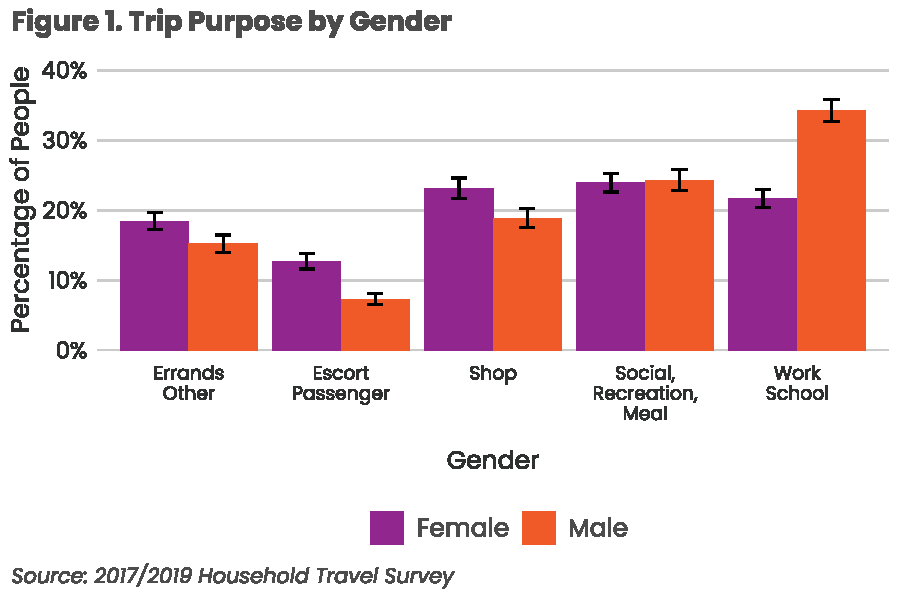
\includegraphics{journal_of_public_transportation_draft_files/figure-latex/trip by gender-1.pdf}

\begin{flushleft}
Women in households with more than two people tend to travel more with other people than men (Figure 2). Transit is often not well set up for people who are traveling with strollers. The walk and bike network are not built out for people of all ages to use.
\end{flushleft}

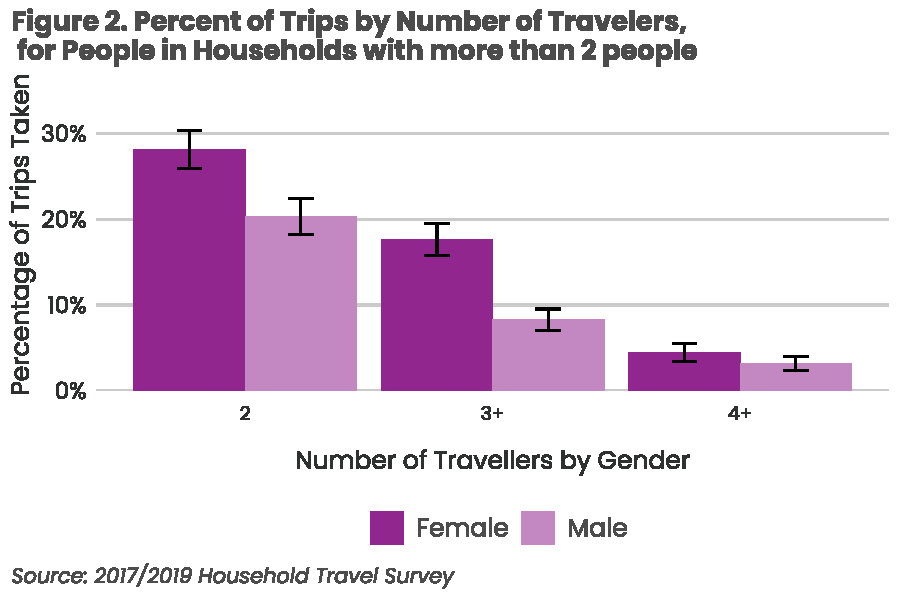
\includegraphics{journal_of_public_transportation_draft_files/figure-latex/Trips by Number of Travellers-1.pdf}
\newpage \pagestyle{otherpages} \setlength{\headheight}{10pt}
\setlength{\textheight}{665pt} \fancyhead[L]{}

\hypertarget{gender-and-race-intersect-in-transportation-needs}{%
\subsection{Gender and race intersect in transportation
needs}\label{gender-and-race-intersect-in-transportation-needs}}

Some women of color experience poverty and low auto ownership in much
higher rates than others. Figure 3 below highlights that some women they
experience greater disparity in earnings across racial groups, but for
other women they experience more disparity across gender. Learn more
about how we can redesign and shape our cities through a more equitable
process in Leslie Kern's book entitled
\href{https://metropolismag.com/viewpoints/leslie-kern-feminist-city/}{\underline{\textcolor{blue}{Feminist City}}}.

\includegraphics{journal_of_public_transportation_draft_files/figure-latex/income race and gender-1.pdf}

\hypertarget{women-of-color-use-transit-most}{%
\subsection{Women of color use transit
most}\label{women-of-color-use-transit-most}}

Women of color in the region used transit on more of their trips than
men and white, non-Hispanic women, prior to COVID-19, as shown in Figure
4. Women of color used transit on nearly double the share of their trips
as compared to white, non-Hispanic women. Women of color most likely
used transit more than white, non-Hispanic women because of having lower
incomes, fewer autos, and living in more transit-friendly areas, but
more data is needed to confirm this hypothesis.

\includegraphics{journal_of_public_transportation_draft_files/figure-latex/unnamed-chunk-2-1.pdf}

\hypertarget{women-bike-commute-far-less-than-men}{%
\subsubsection{Women Bike Commute Far Less than
Men}\label{women-bike-commute-far-less-than-men}}

\begin{flushleft}
Women bike much less than men, regardless or race and ethnicity or income. Some of this is undoubtedly because of bike network design does not feel well-suited or safe for all people of different ages and abilities. There are many considerations as to why women do not feel comfortable riding bicycles as a form of transit, as seen in a study performed by the \href{https://www.itdp.org/2022/07/06/cyclings-gender-gap/}{\underline{\textcolor{blue}{Institute for Transportation and Development Policy}}} in 2022. The inclusion of designated bike lanes, not only that increase comfort and safety for individuals, but that make traveling with children or larger cargo bikes easier would help create more accessibility and user-friendly options. Additionally, increased education about bike routes and access to bikes as a means to developing a biker's comfort and familiarity with bike safety, would help aid in bike commuting ease. 

As a result of some of these considerations not being implemented, in the Puget Sound Region in 2019 only \textbf{6,000} bike trips were made by non-binary folks, and \textbf{30,000} bike trips were made by women, but \textbf{74,000} were made by men (Figure 5). 
\end{flushleft}

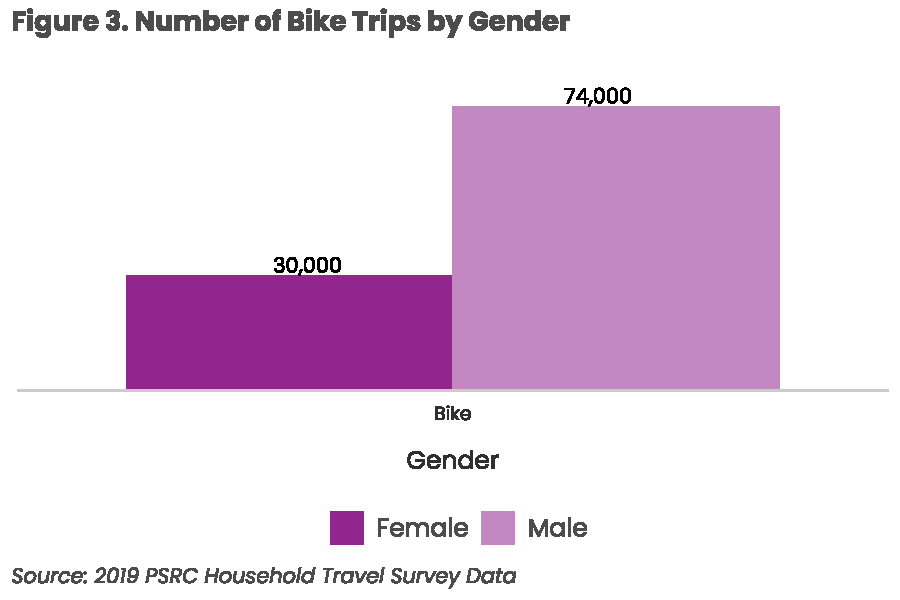
\includegraphics{journal_of_public_transportation_draft_files/figure-latex/Bike trips-1.pdf}

\begin{flushleft}
Not only are certain modalities not conducive to ways in which women move about their environment, but there is also the concern for safety. \href{https://www.itdp.org/2022/07/06/cyclings-gender-gap/}{\underline{\textcolor{blue}{The Institute for Transportation and Development Policy in 2022}}} reported that even though women chose biking less often than men, there was still an active participation in dialogues about how to increase user uptake and accessibility with biking because they deemed it a way to remain safe from harassment or negative transit or walking encounters that they experienced. Women should not have to choose between safety concerns.

How can the transportation and land use system better accommodate older people, household maintenance and caregiving needs? Addressing these questions will improve the system for all genders.
\end{flushleft}

\hypertarget{regional-and-nationwide-data-show-similar-constraints}{%
\subsection{Regional and Nationwide Data Show Similar
Constraints}\label{regional-and-nationwide-data-show-similar-constraints}}

\begin{flushleft}
The findings from \href{https://thesource.metro.net/2019/09/19/metro-releases-understanding-how-women-travel-report/}{\underline{\textcolor{blue}{Understanding How Women Travel}}} about women’s mode choices, how likely they are to travel with others in their care, and their complex trip-chaining patterns could all inform adjustments to Metro’s fare policy to make it more equitable towards women and more cost-competitive with driving and carpooling. Women take shorter more local trips, as opposed to long highway trips. In the Puget Sound Region, women's median trip distance is around 3 miles, whereas men's median trip distance is around 4 miles (source: 2017/2019 Household Travel Survey)Findings about women’s trip purposes and primary responsibility for household errands could all inform the way transit vehicles, transit stations, and bus stops are designed, so that space for traveling with others and carrying  belongings could be better accommodated. Findings about when women are traveling, and average trip lengths could inform new service offerings that meet a mid-day peak travel demand and more local service. 
\end{flushleft}

\begin{flushleft}
Another consideration for amending transit and transportation access is that, women on average, tend to live longer than men, so that at older ages there are many more women who have unique travel needs than men (Figure 8). Women represent a greater share of the older population who needs more specialized transportation services, and less service to work locations.  Older people (who tend to be women more often) have more need for transit in off-peak hours and specialized transportation services. 
\end{flushleft}

\newpage
\pagestyle{otherpages}
\setlength{\headheight}{10pt}
\setlength{\textheight}{665pt}
\fancyhead[L]{}

\hypertarget{changes-brought-about-by-covid-19-pandemic}{%
\subsection{Changes brought about by COVID-19
pandemic}\label{changes-brought-about-by-covid-19-pandemic}}

\begin{flushleft}
Although there were apparent disparities in the 2017/2019 data, COVID-19 brought about abrupt changes to the transportation landscape in 2021. The 2021 Household Travel survey showed big changes in travel behavior. More people were walking and biking, and less people were using transit. Many more people also now had the opportunity to telework. Although women teleworked more than men before COVID-19, the data shows this increase even more in 2021. In 2021, 41\% of women teleworked, as compared to 33\% of men (Figure 7). The difference between telework rates relates to women's job sectors as compared to men, and also household responsibilities. Women of color were about as likely to telework as white, non-Hispanic women.
\end{flushleft}

\includegraphics{journal_of_public_transportation_draft_files/figure-latex/2017/2019 to 2021 charts-1.pdf}

\hypertarget{women-of-color-continued-to-use-transit-more-during-covid-19}{%
\subsubsection{Women of Color continued to use transit more during
COVID-19}\label{women-of-color-continued-to-use-transit-more-during-covid-19}}

Post-COVID-19, people of color continued to use transit more than white,
non-Hispanic people. Women of color were still more likely than white,
non-Hispanic women to ride transit. Most likely the women of color who
still used transit lacked other options, but more investigation is
needed. The largest drop in transit mode shares were for white,
non-Hispanic men.

\includegraphics{journal_of_public_transportation_draft_files/figure-latex/unnamed-chunk-3-1.pdf}

\{\underline{\textbf{Results}}

\{\underline{\textbf{Discussion}}

\hypertarget{trip-purpose-by-gender-20172019-to-2021}{%
\subsection{Trip Purpose by Gender (2017/2019 to
2021)}\label{trip-purpose-by-gender-20172019-to-2021}}

\begin{flushleft}
Not only were there changes in the trips made to work for men and women, but overall trip purpose changed from 2017/2019 to 2021 (Figure 9). COVID-19 brought about an increase in social, recreational, or restaurant/meal pick-ups in 2021 for both men and women, but with women surpassing men in percentage of these trips made. For more information or differences seen in deliveries versus trips made, visit \href{https://www.psrc.org/media/7054}{\underline{\textcolor{blue}{PSRC's website for a more in-depth analysis}}}. Additionally, although it appeared as though women made less trips escorting additional family members (from 13\% to 8\%), men's trips remained at about 7\%, which means that overall trips changed, possibly due to the increase in women's telecommute behaviors or lack of activities outside of the home. Overall, women made more trips than men in all other categories besides work or school trips. 
\end{flushleft}

\includegraphics{journal_of_public_transportation_draft_files/figure-latex/2017/2019 to 2021-1.pdf}

\{\underline{\textbf{Conclusions}}

\hypertarget{conclusion}{%
\subsection{Conclusion}\label{conclusion}}

\begin{flushleft}
With increased emotional labor and care-taking demands, and with women more likely to live in poverty and having less employment and lower incomes than men, there are many aspects of transit and transportation modalities that need to be reassessed to support women's needs. Women of color need a robust transit network with more reliable service throughout the day. Biking, walking, and transit don't always feel accessible or safe, and access to a vehicle isn't always available to women. While an increase in telework has removed some of the additional burden to trip-chaining for women, we need to consider how we create and manage transportation so that it may be equitable to all. Transit especially needs to be designed around women of color, since they use transit more than other groups.

While we are working towards a more non-binary understanding of gendered data, we acknowledge that much of the data presented above does analyze information and patterns in a binary manner.

\href{https://www.psrc.org/media/7505}{\underline{\textcolor{blue}{Download the data used in this Trend}}}. 

{\underline{\textbf{Appendices}}

{\underline{\textbf{References and Citations}}

\end{flushleft}

\end{document}
